\section{Technische Umsetzung}
In diesem Kapitel wird die Umsetzung des modellierten Systementwurfs als prototypische Implementierung im Detail beschrieben. Es gibt einen Einblick in den Prozess der Konfiguration eines Blockchain Netzwerks, das mehrere Unternehmen umfasst. Dabei wird Eingangs auf die zugrunde liegende Architektur des Business Netzwerks bezug genommen. Aufbauend auf dem Fundament des Business Netzwerks werden Geschäftslogik und Berechtigungssystem erläutert.

\subsection{Business Netzwerk}
Als Basis des Blockchain Systems dient ein Hyperledger Fabric Netzwerk. Alle Dienste des Netzwerks werden in einer virtualisierten Umgebung bereitstellt. Dazu wird die Container Technologie von Docker\footnote{Docker basiert auf Linux Techniken wie \textit{Cgroups} und \textit{Namespaces}, um isolierte Umgebungen innerhalb eines Hostsystems bereitzustellen \citep{Bengel2008,Oeggl2019}.} verwendet. Zum einen bietet sich die Container Technologie zur Umsetzung eines Prototyps an, da sie sehr viel flexibler und leichtgewichtiger ist als die konventionelle Virtualisierung über Virtuelle Maschinen \citep{Ahmed2018}. Zum anderen sind die Basis Komponenten zum aufspannen eines Hyperledger Fabric Netzwerks bereits von der Linux Foundation als Container Abbild bereitgestellt, was die Realisierung des Prototypen signifikant beschleunigt. Im folgenden wird die technische Umsetzung eines Peer Knotens mittels Docker beispielhaft beschrieben. Die anderen Systemkomponenten (siehe Kapitel \ref{system-design-concept}) verhalten sich vom Aufbau her äquivalent zu einem Peer Knoten, sie sind lediglich unterschiedlich konfiguriert um verschiedene Aufgaben auszuführen. Die Netzwerke beider Unternehmen werden in diesem Fall auf der selben Maschine betrieben. In einem produktiven Umfeld würde jedes Unternehmen seine eigene Umgebung bereitstellen.

Das Prototyp Netzwerk umfasst zwei Organisationen: \textit{Org1} und \textit{Org2}. Das Unternehmen \textit{Org1} verwendet den Domänennamen \textit{org1.example.com}. Der \acf{msp} für \textit{Org1} wird als \textit{Org1MSP} bezeichnet. Das Unternehmen \textit{Org2} verwendet den Domänennamen \textit{org2.example.com}. Der \acf{msp} für \textit{Org2} heißt \textit{Org2MSP}.

\paragraph{Netzwerk Komponenten}$~~$\\
Das Hyperledger Fabric Netzwerk besteht insgesamt aus den folgenden Komponenten und Schnittstellen:

\begin{itemize}
    \item Zwei Peer Knoten für \textit{Org1}
    \begin{itemize}
        \item \textit{peer0.org1.example.com}
        \item \textit{peer1.org1.example.com}
    \end{itemize}
    \item Eine \ac{ca} für \textit{Org1} (\textit{ca.org1.example.com})
    \item Zwei Peer Knoten für \textit{Org2}
    \begin{itemize}
        \item \textit{peer0.org2.example.com}
        \item \textit{peer1.org2.example.com}
    \end{itemize}
    \item Eine \ac{ca} für \textit{Org2} (\textit{ca.org2.example.com})
    \item Ein einzelner Orderer Peer (\textit{orderer.example.com})
\end{itemize}

\noindent
Jede dieser Komponenten stellt einen Docker Container dar und ist auf Netzwerkebene über seinen Hostnamen ansprechbar. Die gesamte Netzwerkkommunikation ist über das \ac{tls}-Protokoll\footnote{\ac{tls} ist ein hybrides Verschlüsselungsprotokoll, um Datenübertragungen vor Angriffen zu schützen \citep{RFC5246}.} abgesichert. Aus diesem Grund müssen alle Zertifikate der \ac{ca} auf dem Hostsystem zur Verfügung stehen, damit eine Kommunikation mit dem Netzwerk stattfinden kann. Für Organisation \textit{Org1} ist ein Administrator User angelegt mit Namen \textit{Admin@org1.example.com}. Ebenfalls ist für Organisation \textit{Org2} ein Administrator User angelegt der \textit{Admin@org2.example.com} heißt. Zusätzlich zu den Administrator Usern der Organisationen ist die \ac{ca} mit einem Standard User konfiguriert. Der \ac{ca} User besitzt im gegensatz zu den Administrator Usern keine Berechtigungen, um Smart Contracts (Chaincode) auf Peers des Netzwerk zu installieren. Damit die Peer Administatoren sich mit dem Netzwerk verbinden können wird ein Verbindungsprofil benötigt. In diesem Verbindungsprofil werden alle Komponenten des Netzwerks definiert und die zugehörigen \ac{tls} Zertifikate hinterlegt (siehe Anhang \ref{lst:connection-profile}). Verbindungsprofil und die digitale Identität des Administrator Users, bestehend aus Zertifikat und privatem Schlüssel, bilden zusammen die sogenannte \textit{Business Network Card}. Hiermit kann sich der Administrator User über eine Hyperledger Fabric \ac{cli} mit dem Netzwerk verbinden und Befehle absetzen.

\begin{figure}[H]
	\centering
	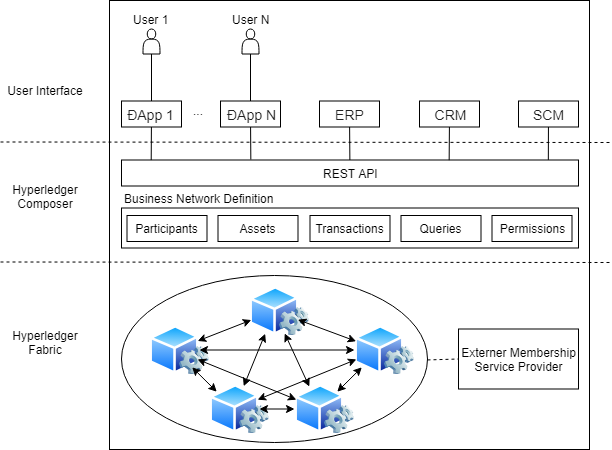
\includegraphics[width=1\linewidth]{pictures/poc-food-chain-traceability}
	\caption[Gesamtsystem Prototyp]{Gesamtsystem Prototyp}
	\label{fig:poc-food-chain-traceability}
\end{figure}

Nachdem starten der Docker Container lässt sich ein einfacher Smoke Test\footnote{Mit einem Smoke Test sollen grundlegende Probleme bei einer Software oder einem System offengelegt werden, bevor die Entwicklung von folge Komponenten begonnen wird \citep{Everett2007}.} durchführen, um sicherzustellen das das Netzwerk ordnungsgemäß hochgefahren wurde und alle Knoten arbeiten. Docker bietet zum Mangement der Container ein \ac{cli} an. Hiermit lässt sich der Smoke Test mit einem Einzeiler auf dem Terminal ausführen. Damit ist die Basiskonfiguration des Systems abgeschlossen und das Peer Netzwerk ist aufgespannt (siehe Abbildung \ref{fig:poc-food-chain-traceability} Abschnitt \textit{Hyperledger Fabric}). Im aktuellen Zustand kann das Netzwerk noch keine Transaktionen erzeugen oder verarbeiten. Dazu muss erst noch die im nächsten Kapitel beschriebene Geschäftslogik durch einen Administrator User auf einem Peer Knoten des Unternehmens installiert und instantiiert werden.

\subsection{Smart Contracts}
Smart Contracts heißen im Hyperledger Model \textit{Chaincode}. Sie setzen sich aus vier Elementen zusammen. Model, Logik, Zugriffskontrolle und Abfragedefinition bilden das sog. \acf{bna}. Das \ac{bna} lässt sich in jedes mit Hyperledger Fabric aufgespannte Blockchain Netzwerk deployen. Die Funktionsweise eines Smart Contracts soll hier am Beispiel des Eigentumswechsels eines Materials näher erläutert werden. Dazu wird auf jedes der vier Elemente eines \ac{bna} eingegangen, um den strukturellen Aufbau zu zeigen. Im Sinne des Models werden ein \textit{Participant}, ein \textit{Asset} und eine \textit{Transaction} definiert wie in Listing \ref{lst:example-model-definition}. Die eigentliche Verarbeitungslogik wird gesondert von der Datenstruktur definiert (Listing \ref{lst:transaction-logic-change-ownership}). In diesem Fall wurde die Logik in der Programmiersprache JavaScript implementiert.

\begin{lstlisting}[caption={Model Example Definition},label=lst:example-model-definition]
namespace io.dev.foodchain

abstract participant Company identified by gln {
    o String gln
    o String name
}

participant Farmer extends Company {}

asset Material identified by materialId {
    o String materialId
    --> Company owner optional
}

transaction changeMaterialOwnership {
    --> Material material
    --> Company newOwner
}
\end{lstlisting}

Zeile 1 in Listing \ref{lst:example-model-definition} definiert einen Namensraum für das gesamte Model. In einem produktiven Scenario würde ein Model erheblich größer sein, als das im Prototyp verwendete vereinfachte Model. Damit bei steigender Komplexität des abzubildenden Models Überblick und Wartbarkeit erhalten bleiben lässt sich das Model über mehrere Dateien abbilden und über den Namensraum auf logischer Ebene miteinander verknüpfen. Zeile 3 bis einschließlich Zeile 6 zeigt die Definition der abstrakten Klasse \textit{Company} vom Typ \textit{Participant}. Diese Definition wird in Zeile 10 konkret ausgeprägt durch die Klasse \textit{Farmer}. Äquivalent dazu werden auch alle anderen Teilnehmer der Wertschöpfungskette implementiert. Zeile 10 bis Zeile 14 zeigt die Implementierung des Assets \textit{Material}. Über die Eigenschaft \textit{owner} (Zeile 12) wird ein \textit{Material} später immer einem eindeutigen Besitzer zugeordnet. Die Eigenschaft \textit{owner} wurde dabei als direkte Ressourcenverknüpfung implementiert. Eine Ressourcenverknüpfung im Hyperledger Model lässt sich mit einer Fremdschlüsselbeziehung in einem relationalen Datenbankschema vergleichen. Die Eigenschaft kann in diesem Fall nur Werte annehmen die eine gültige Ausprägung der abstrakten Klasse \textit{Company} sind und damit auch allen konkreten Ausprägungen dieser Klasse. Um das Beispiel einfach und verständlich zu halten wurden die Definitionen der \textit{Participants} und \textit{Assets} in verkürzter Form abgebildet. Das vollständige Prototypen Model befindet sich im Anhang.

% 1.2.2 Adding JavaScript transaction logic\\
\begin{lstlisting}[caption={Transaction Processor Function \textit{changeMaterialOwnership(tx)}},language=ES6,label=lst:transaction-logic-change-ownership]
/**
* Change material ownership transaction
* @param {io.dev.foodchain.changeMaterialOwnership} tx
* @transaction
*/
async function changeMaterialOwnership(tx) {
    // input parameter
    const oMaterial = tx.material;
    const oNewOwner = tx.newOwner;
    const oActualOwner = tx.material.owner;

    // checks
    //// check if proposed input material exists
    const oMaterialRegistry = await getAssetRegistry(NS + '.Material');
    const bMaterialExists = await oMaterialRegistry.exists(oMaterial.getIdentifier());
    if(!bMaterialExists) {
        throw new Error('Input material "' + oMaterial.getFullyQualifiedName() + '" does not exist.');
    }
    //// AND belong to tx issuer (should be checked by permissions file)
    if (oMaterial.owner !== getCurrentParticipant()) {
        throw new Error('You are not allowed to change asset: "' + oMaterial.getFullyQualifiedName() + '".');
    }
    //// check if proposed new owner exists
    const oParticipantRegistry = await getParticipantRegistry(oNewOwner.getNamespace());
    const bNewOwnerExists = await oParticipantRegistry.exists(oNewOwner.getIdentifier());
    if(!bNewOwnerExists) {
        throw new Error('New owner "' + oNewOwner.getFullyQualifiedName() + '" does not exist.');
    }

    // business logic
    //// put actual owner to the history stack
    oMaterial.ownerHistory.push(oActualOwner);
    //// set new owner for asset
    oMaterial.owner = oNewOwner;
    //// update asset registry
    await oMaterialRegistry.update(oMaterial);

    // event emitting
    //// create and emit default tx event


    // set return value

}
\end{lstlisting}

%1.2.3 Adding access control\\

\begin{lstlisting}[caption={Berechtigungsdefinition},label=lst:model-permissions]
rule OwnerHasFullAccessToTheirAssets {
    description: "Allow all participants full access to their assets"
    participant(p): "io.dev.foodchain.*"
    operation: ALL
    resource(r): "io.dev.foodchain.*"
    condition: (r.owner.getIdentifier() === p.getIdentifier())
    action: ALLOW
}
\end{lstlisting}

%1.2.4 Query definition\\

\begin{lstlisting}[caption={Abfragedefinition},label=lst:model-permissions]
query selectMaterialsWithBonusCondition {
  description: "Select materials based on bonus condition"
  statement:
      SELECT io.dev.foodchain.Material
          WHERE (bonus == true)
}
\end{lstlisting}

% 1.3 Generate a business network archive\\
% 1.4 Deploying the business network\\
% 1.4.1 Retrieving the credentials\\
% 1.4.2 Deploying the business network\\
% 1.5 Generating a REST Server\\

\subsection{User Interface}
1. SAP Build\\
2. SAPUI5

\subsection{Zusammenfassung technische Umsetzung}



\newpage
